\chapter{Introduction}
\label{chapter_1}

\begin{abstract}
This is the abstract of the introduction
\end{abstract}

\newpage

\section{Light Microscopy}
\dropcap{M}{icroscopes} have become an indispensable tool in all research fields
in which there is the need to look at small features. The first microscopes
developed by Antoni Van Leeuwenhoek in the XVII century were aimed at studying
fabrics; it didn't take long however to discover that nature was hiding amazing
elements beyond what the bare human eye could see. The first microscopes focused
into developing better lenses and clever illumination schemes. 

With the development of the ondulatory theory of light a fundamental limitation
for optical microscopes appeared: the diffraction limit. Abbe realized that no
matter how good a lens is, there will always be a limit to how much it is
possible to focus light. This limit is determined mainly by the wavelength of
the employed light beam and by the maximum angle the lens is able to focus. 

The diffraction limit puts a restriction to the size of the features that can be
studied under an optical microscope. The use of shorter wavelengths, as
X-rays\cite{von1915concerning} opened the possibility to investigate much
smaller structures. However this strategy is limited to very well defined
periodic structures, such as crystals. Soft matter samples including cells and
polymers would therefore be out of the scope of these techniques.

Fluorescence was first observed and characterized during the second half of the
$19$th century. But only several decades later, around $1930$, the first
applications of fluorophores to stain biological samples started to emerge. They
were highly specific, allowing to easily detect tissue components or bacteria.
The wealth of information that could be retrieved thanks to fluorescence was
fundamental for the development of the fluorescence microscope as a standard
tool in almost any biological or material science laboratory. However normal
fluorescence microscopy does not overcome the diffraction limit.

It was only at the end of the XX century that a major breakthrough occurred in
the field of optics: the detection of a single-molecule fluorescence by M.
Orrit and J. Bernard\cite{PhysRevLett.65.2716}. Single-molecules opened the door
to studying materials with unprecedented spatial resolution, but also to determine properties that
would have been hidden by bulk broadening. The first studies were done at low
temperature (few Kelvins) and allowed to determine properties not only of the
fluorescent molecules but also of the hosting matrices, mainly polymers and
crystals.

With a growing interest in the field, a big effort was placed in allowing the
detection of single-molecules at room temperature. This led to the development
of new organic dyes and to establish single-molecule fluorescence microscopy as
one of the cornerstones of many research fields. Localization of single
fluorophores led to the development of what is now known as super resolution
microscopy\cite{moerner2015single}. By carefully determining the centroid of the
emission pattern, it is possible to determine the position of a molecule with
higher accuracy than what the diffraction limit would allow\cite{Moerner2007}.

Molecules however show two phenomena known as blinking and bleaching. At room
temperature it is impossible to prevent fluorophores from going to dark states,
meaning that their fluorescence signal will disappear. In the case of blinking
it happens for short periods of time and hence the name. If the molecule
undergoes a non reversible transition to a dark state, it will be called
bleaching. This puts a hard limit to the experiments that can be performed
employing single-molecules, since they cannot be observed for extended periods
of time. Tracking is limited to few seconds, imaging is limited to few frames or
to cleverly engineered illumination strategies.

As single-molecule detection allowed to bridge the length mismatch between
visible light and biologically relevant scales, new agents that can fill the gap
between biologically relevant time scales and fluorophores' observation times
are of utmost importance. In this direction different approaches were taken,
including employing scattering instead of
fluorescence\cite{ortega2012interferometric}, the use of semiconductor quantum
dots\cite{alivisatos2005quantum} and of metallic
nanoparticles\cite{huang2009gold}. The latter are the focus of this thesis and
of the next few sections.

\section{Gold Nanoparticles}
Metallic nanoparticles have been utilized for a very long time. In a fortuitous
way Romans managed to generate red-coloured glass by dispersing gold nanospheres
into their glass mixing strategies; the beautiful Lycurgus
cup\cite{barber1990investigation} is the only surviving complete example of such
technique, together with some other glass fragments of the time. Nanoparticles
in the glass preserved their optical properties for centuries, however the
explanation of the phenomenon came several centuries later.

Gustav Mie in $1908$ calculated the scattering of a plane wave incident on
spherical particles\cite{mie1908beitrage}. It relies on fully solving Maxwell
equations and nowadays it is simply known as Mie scattering. In the original
paper it is possible to observe the measured and calculated scattering spectra
of gold nanospheres. Both experiments and theory show a peak at around $550\nm$;
because of the weaker interaction with light of longer wavelengths, the reddish
color of colloidal gold nanoparticles can be explained.

The peak observed is related to a resonance of the oscillating conduction
electrons on the surface of the metal and is known as plasmon resonance. For
particles much smaller than the incident wavelength, a simplification of the Mie
formalism can be made by considering only the first order. In this case the
polarizability of a nanosphere is given by\cite{bohren2008absorption}

\begin{equation}\label{eqn:polarizability}
	\alpha_{\textrm{sphere}} =
	3\epsilon_0V\frac{\epsilon(\omega)-\epsilon_m}{\epsilon(\omega)+2\epsilon_m}
\end{equation}

\noindent where $\epsilon_0$ is the permittivity of vacuum, $\epsilon(\omega)$
is the permittivity of the metal as function of incoming excitation frequency $\omega$
and $\epsilon_m$ is the permittivity of the surrounding medium. The absorption
cross section can thus be calculated as
$\sigma_\textrm{abs}=k\textrm{Im}(\alpha)$ and the scattering as
$\sigma_\textrm{scatt}=k^4|\alpha|^2/(6\pi)$.

From equation \ref{eqn:polarizability} it is possible to see that a resonance
will appear when $\textrm{Re}(\epsilon(\omega)) = -2\epsilon_\textrm{m}$. It is
important to note that the energy at which this resonance appears is therefore
dependent not only on the particle's material properties but also on the
surrounding medium's optical constants. In the case of elongated nanoparticles,
some correction factors can be introduced to the polarizability. However several
computer packages\cite{Yurkin2011,oskooi2010meep,draine2013user} exist to
calculate with a great precision absorption and extinction cross sections of
arbitrary geometries and therefore it is not worth entering into the specifics
of the calculations\footnote{A complete description of how to calculate the
plasmon resonance can be found at:\newline
https://www.aquicarattino.com/science/plasmon-resonance/}.

\begin{sloppypar}
It is important to point out however that while nano spheres have resonances
that slightly change with their radius, elongated particles such as nanorods
present a longitudinal resonance that strongly depends on their aspect ratio.
The more elongated particles will have resonances with lower energies (or
conversely with longer wavelengths). Moreover particles with resonances to the
near infrared region show a narrower resonance\cite{Sonnichsen2002}, making them
interesting candidates for sensing applications. In biological conditions this
is particularly relevant, since cells are typically transparent to near infrared
wavelengths.
\end{sloppypar}
\begin{sloppypar}
A standard procedure to obtain gold nanoparticles is through wet chemical
methods\cite{Vigderman2012}. Even in the best of cases there will be a
dispersion in shapes in the sample. The differences between nanoparticles can be
observed with electron microscope micrographs, but also optically. Slightly
different particles will show different resonances\cite{Lindfors2004}, and this
is more significant when working with elongated particles. On one hand this
simplifies the identification of dimers or clusters, since more than one
resonance peak will be observed. On the other it means that in any given sample
there will be a distribution of resonances and therefore it is simple to
characterize phenomena that depend on the energy of the plasmon resonance
without the need to change the sample.
\end{sloppypar}
It is important to note that besides the geometrical factors, nanoparticles also
show a broad distribution of their quantifiable properties. For example the
quantum yield of nanoparticles that are apparently equivalent (similar in size,
same resonance energy) can differ from each other in almost an order of
magnitude\cite{Yorulmaz2012}. In every chapter of this thesis the variation from
particle to particle can be observed for phenomena ranging from chemical
etching\cite{Carattino2016} to electron-phonon coupling.

\section{Luminescence from gold nanoparticles}
\label{sec:luminescence}
Light emission from gold and copper was first observed by
Mooradian\cite{Mooradian1969} in $1969$. In his work, electron and holes in the
metal were excited with visible light and the emission was observed at longer
wavelengths. Strikingly, the emission quantum yield (i.e. the number of emitted
photons per absorbed photon) that he estimated was in the order of $10^{-10}$.
In subsequent years several studies showed that this low number could be
increased with the presence of sharp edges\cite{boyd1986photoinduced} or
tips\cite{Mohamed2000}, but still it would be much lower that what is observed
for an organic dye, in the order of few percent at least.

When transitioning from bulk gold to nanoparticles, the interaction of light
with metals will be highly influenced by the presence of the plasmon
resonance\cite{Dulkeith2004}. On one hand nanoparticles will have large
absorption cross sections in specific wavelength regions, as explained in the
previous section. On the other hand the emission spectrum will be also
concentrated around the plasmon resonance. Previous works have shown a big
overlap between the scattering and the emission spectra of gold nanoparticles.

The emission quantum yield of single gold nanoparticles can be several orders of
magnitude higher than bulk values partly due to the presence of sharper edges.
Typical quantum yield values are in the order of $10^{-6}$\cite{Yorulmaz2012},
several orders of magnitude lower than single organic dye molecules, but the
absorption cross section can be in the order of $10^{-2}\um^2$, $6$ orders of
magnitude higher than those of dye molecules. The combination of both factors
makes it possible to use luminescence to detect single gold nanoparticles in a
standard fluorescence microscope.

The photoluminescence of gold nanoparticles can be excited mainly through two
different approaches. It is possible to use a short wavelength laser, as a
$532\nm$ to excite interband transitions in gold\cite{Beversluis2003a}, as well
as the transverse plasmon resonance if working with rods. The emission from
particles can be collected after placing a notch or long pass filter in the
detection path to prevent the excitation light to reach the detectors.
Illuminating with a short wavelength allows to collect the entire plasmonic
emission, but doesn't fully exploit the advantage of the larger absorption cross
section that the resonance provides.

Another approach to observe luminescence from nanoparticles is therefore to
excite them close to their resonances. In this way it is possible to benefit
from the higher absorption cross section allowing to lower the excitation
powers. Recent studies have shown that the emission quantum yield does not
change between exciting with shorter wavelengths or at the resonance of the
particles\cite{Cheng2015}. However the photoluminescence itself is also coupled
to the plasmon; if excited in resonance, the emission will be concentrated
around the excitation wavelength\cite{Sundararaman2014}. The presence of
detection filters will therefore block an important part of the emission
spectrum.

For many purposes it is possible to compare dye molecules to gold nanoparticles.
Since they emit light at different wavelengths than the excitation it is
possible to achieve a high spectral selectivity when observing them in a
fluorescence microscope. However there is an important difference between both
when looking at the Stokes shift of their emission. Nanoparticles excited close
to or at the resonance emit light around the excitation wavelength and therefore
the Stokes shift is small. Compared to molecules that have defined electronic
energy levels, in gold nanoparticles the energy levels of electrons can be
considered as a continuum. 

Normally the Stokes shift can be conceptualized as conservation of energy: a
photon of a given energy excites the electrons of a material that subsequently
relax back by emitting another photon, by transferring energy in the form of
heat to the medium or a combination of both. It is expected therefore that the
emitted photon has a lower energy than the incident one. This is always valid
unless the excited electrons can somehow gain energy from the medium before
relaxing back radiatively. If this happens, the processes called Anti-Stokes
and the emitted photons possess a higher energy than the excitation.

When excited in resonance, gold nanoparticles exhibit anti-Stokes luminescence
with intensities that can be compared to the Stokes shifted emission. In brief,
the mechanism proposed for the emission of photons with higher energies is the
interaction of electron and holes with phonons in the gold lattice before
recombining radiatively. Assuming that the anti-Stokes emission from gold
nanoparticles depends only on the population of phonons, the general shape of
the emission is expected to be

\begin{equation}\label{eqn:antiStokes}
	\bar{I}\approx\left(\exp\frac{\hbar\omega}{k_bT}-1\right)^{-1}.
\end{equation}

\noindent where $\omega$ is the frequency of the emitted photon, $k_b$ is
Boltzmann constant and $T$ is the temperature. 

Notably in equation \ref{eqn:antiStokes} the only free parameter for adjusting
is the temperature. If properly characterized, the anti-Stokes emission
spectrum should provide a way to estimate the absolute surface temperature of
the particles without any previous calibration. 

\section{Applications of gold nanoparticles}
\subsection{Tuning the resonance of gold nanoparticles}
The previous two sections highlighted different strategies for detecting single
gold nanoparticles as nanospheres or nanorods. The principal characteristic of
the particles is the presence of a localized surface plasmon resonance.
The resonance wavelength (or energy) will be given by the geometry of the
particle and by the surrounding medium's properties, such as the refractive
index or temperature. Normally the geometry is determined during the synthesis
procedure and thus the resonance is fixed after immobilizing the particles on a
substrate.

Chapter \ref{ch:KCN} focuses into tuning the plasmon resonance \textit{in-situ},
once they are immobilized on a substrate and optically characterized. Currently
two approaches exist for tuning the plasmon resonance after synthesis: ($1$) it
is possible to tune the refractive index of the medium using an electric or
magnetic field\cite{Kossyrev2005}. ($2$) It is possible to induce shape
modifications of the nanoparticles either through
chemical\cite{Jana2002,Rodriguez-Fernandez2005,Carbo-Argibay2007,Tsung2006,Ni2008}
or physical means\cite{Link2000,Horiguchi2008,Yorulmaz2012}. 

In the majority of the reports a blue-shift of the plasmon resonance has been
observed. This means that gold nanorods reshape into spheres, or that edges with
higher curvature are softened after chemical etching. For physical processes, as
thermal reshaping after excitation with a high-intensity laser this can be
explained through a rearrangement of surface atoms to energetically more
favorable configurations. In the case of chemical etching, previous works have
always focused on bulk measurements in suspension. The tips of the particles
tend to be more reactive because they are less protected by surfactants. 

Chapter \ref{ch:KCN} shows that through well known chemistry between gold and
cyanide ions it is possible to induce a red-shift of the plasmon. This is
modelled through an isotropic etching of the particles, obtaining a good
agreement between the calculations and the experiments. The main difference with
previous works is the absence of a capping agent on the particles' surface.
Controllably changing the shape of nanoparticles is of great importance for
experiments where a specific resonance is needed. 

\subsection{Imaging through detection of anti-Stokes emission}
Gold nanoparticles are ideal candidates for labelling of biological samples
because they prove to be innocuous to the cell\cite{Lewinski2008} but also
because they can be observed for extended periods of
time\cite{PEREZJUSTE2005,Mohamed2000}. The big drawback of gold nanoparticles is
their low quantum yield. Since the absorption cross section of the particles
scales as their volume, detecting smaller particles in presence of background
requires a specific approach.

To overcome these difficulties, several techniques have been developed for
imaging gold nanoparticles, including two-photon excited
luminescence\cite{VandenBroek2013}, photothermal \mbox{heterodyne}
detection\cite{Berciaud2006} and interferometric detection\cite{Ignatovich2006}.
Each of these methods is useful but their operation requires dedicated setups
and a high level of expertise.

Chapter \ref{ch:Imaging} of this thesis shows that it is possible to image gold
nanorods in biologically relevant conditions through detection of the
anti-Stokes emission. By placing a short-pass filter in the detection path the
background level is reduced significantly, while the luminescence signal from
the particles remains high. This is valid even in the presence of cells stained
with $\atto$, a high quantum yield dye. In this conditions it is not possible to
observe any single nanoparticle through conventional Stokes-shifted emission 
while the anti-Stokes scheme presents signal-to-background ratios of more than
$10$.

The technique presented in chapter \ref{ch:Imaging} can be readily implemented
in any conventional microscope by the addition of the appropriate filters. It
does not require any special operation nor infrastructure. Moreover any data
analysis tool for tracking, imaging, centroid extraction, etc. can readily be
implemented without further modifications. 

\subsection{Gold nanoparticles as nano-Thermometers}
\begin{figure}[htp]
 \centering
 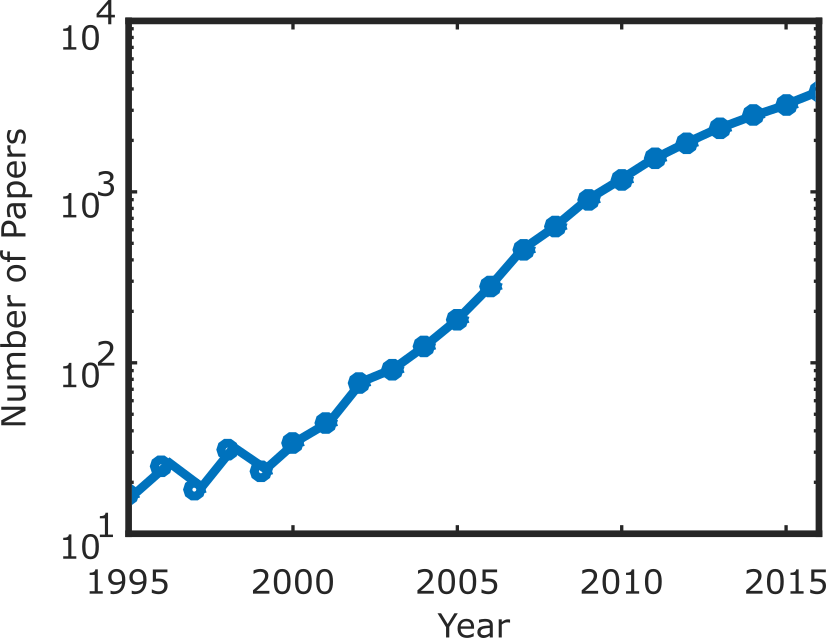
\includegraphics[width=0.40\textwidth]{Chapters/01_Introduction/Figures/paper_PT_therapy.png}
 \caption{Number of papers published containing the terms Plasmonic Photo
 Thermal Therapy since 1995. Note the logarithmic scale in the y-axis.}
 \label{fig:PPTT}
\end{figure}

During the past two decades there has been an increasing interest in gold
nanoparticles as possible agents for medical
treatments\cite{Gobin2007,Huang2006,Huo2014}. The strong interaction between
particles and light makes them ideal candidates not only for labelling but also
for dissipating heat into very localized environments
\cite{Huang2008,Huang2006,Gobin2007,Hirsch2003}.
This simple approach can be used for instance to induce death of cancer cells
and is normally referred to as Plasmonic Photo Thermal Therapy (PPTT). Figure
\ref{fig:PPTT} shows the number of papers published in this field since $1995$.
The more-than-exponential increase serves as a measure for the relevance this
technique is gaining.

After decades of research there is however almost no information regarding the
temperatures that need to be reached by the nanoparticles to induce cell death.
Much less is available at a single-particle/single-cell level. Moreover the
field of thermometry at the nanoscale is subject to a moderate
debate\cite{Yang2011a,Suzuki2015} since some experimental
findings\cite{Yang2011a} contradict expected values from thermodynamic
considerations\cite{Sato2014}.

Chapter \ref{ch:AntiStokes} of this thesis focuses into the characterization of
the mechanisms that give raise to anti-Stokes luminescence. Discarding
multi-photon processes, photons with higher energies than the excitation energy
require interactions with thermal baths. In a nanoparticle electron and holes
can interact with phonons before recombining radiatively, as discussed in
section \ref{sec:luminescence}.

By carefully fitting the luminescence spectra of single gold nanorods and
nanospheres it is possible to extract the surface temperature of the particles.
The method presented in chapter \ref{ch:AntiStokes} does not depend on any
ad-hoc calibration and can be performed in any confocal microscope with a
coupled spectrometer. The chapter shows the increase in temperature with
increasing laser powers and also shows the changes that the luminescence spectra
undergo when increasing the medium's temperature.

The results from the chapter can have a significant impact on an emerging
community that addresses one of the most pressing health issues of this
time.

\subsection{Plasmon damping as function of temperature}
Luminescence is not the only strategy of detecting gold nanorods with an optical
microscope. Gold nanoparticles have a large scattering cross section coinciding
with the plasmon resonance. If excited with a white light source it is possible
to record the scattering spectra without much inconvenience. The resonance
itself is affected by the surrounding conditions\cite{Liu2009b,Konrad2013}. For
instance changes in refractive index of the medium induce changes in the
resonance position, while different temperatures of the particles will show
different plasmon damping rates.

In principle there are four main mechanisms responsible for the damping of the
plasmons\cite{Sonnichsen2002,Novo2006,Hu2008}: electron-phonon coupling,
electron-surface interactions, electron-electron collisions and radiative
damping. Out of those only the coupling with phonons shows an appreciable
dependence on temperature\cite{Liu2009b,Konrad2013}. Therefore studying the
dependence of the plasmon width with temperature can provide an alternative way
of measuring temperature.

Chapter \ref{ch:Damping} focuses on the characterization of the plasmon
resonance of single gold nanorods at various temperatures. The plasmon width
increases linearly with temperature, as predicted from the Debye model of
phonons. Measuring the broadening of the resonance can then be related to
changes in temperature of the surrounding medium. 

Employing the scattering signal not only benefits from the high cross section of
the particles, it also prevents to induce a temperature increase because of
higher laser excitation powers. However the broad distribution of widths and
broadening rates found in the studies of chapter \ref{ch:Damping} does not allow
to perform an absolute temperature measurement but to measure a relative change.
This is similar to other experiments performed with quantum dots and therefore
expand the toolbox of available techniques for thermometry at the nanoscale.

\section{One program to rule them all}
All modern laboratories rely on computer equipment to perform measurements,
ranging from integrated micro controllers to supercomputers. The first, for
example, is responsible for maintaining a stable temperature of a heating plate;
the latter on the other hand can analyze data online in high throughput
experiments and take decisions on the fly as happens in the popular
multi-billion euro experiments. However for the average experimentalist there is
a big gap between what is needed and what is available.

Flexible, open source programs to control experiments are hard to find in the
internet. This generates a double negative effect: researches find themselves
reinventing the wheel more often than desired. A simple home built confocal
microscope requires a dedicated computer program to run but it can take months
to develop. Readily available software normally lacks the flexibility that new
science needs, limiting the creativity of researches while planning
experiments.

All the chapters of this thesis relied on a flexible computer program that
allowed to perform tasks in an automated fashion. A direct consequence of this
is an increase in the throughput of the setup with experiments running over
night, for example. It also allowed to perform experiments that wouldn't have
been possible without a computer assisted strategy. 

The computer program has been made open source and can be found on Github. It
started to be developed for simplifying repetitive tasks as refocusing on a
particle or triggering a spectrometer. But it evolved into a fully functional
GUI for performing and visualizing $2$D and $3$D scans, acquiring fast
timetraces, monitoring an optical tweezer and communicating with serial devices
as well as over the network. The latest developments of the software allow to
define API's for easy integration with applications on smartphones or to control
several independent setups through the network (including through the internet).

Chapter \ref{ch:KCN} shows results where several particles were analyzed in an
iterative way while being etched with potassium cyanide. Refocusing on the
particles by hand is too slow for processes that happen as fast as the ones
shown in the chapter. The program allowed to refocus on selected particles and
trigger a spectrometer without user interaction. 

Chapter \ref{ch:Imaging} shows the scanning capabilities of the software for
imaging purposes. Moreover the specific program for acquiring the power
dependence plots can be written in about $20$ lines of code. When varying the
temperature of the sample as in chapters \ref{ch:AntiStokes} and
\ref{ch:Damping} it is of utmost importance being able to refocus on a reference
particle to compensate for the drift of the setup.  

The software even if developed with an optical microscope in mind, can be easily
extended to other configurations. The choosing of Python as the programming
language provides platform independence; it can run without inconvenience on
several Windows versions, Mac OS and Linux. The main objective of the program is
to provide a lower level layer on which to build creative solutions to complex
problems.

\references{Chapters/01_Introduction/introduction}